\documentclass[conference]{IEEEtran}

\usepackage{amsmath}
\usepackage{booktabs}
\usepackage{graphicx}
\usepackage{url}
\usepackage[hidelinks]{hyperref}

\title{Evaluating Logical Reasoning in Large Language Models Through Fine-Tuning and Neuro-Symbolic Bridging}

\author{\IEEEauthorblockN{Anonymous Author(s)}
\IEEEauthorblockA{Anonymous submission}}

\begin{document}
\maketitle
\begin{abstract}
Large language models (LLMs) perform well on many language tasks but remain unreliable at multi-step deduction over explicit facts and rules. Two remedies are usually pursued separately: task-specific fine-tuning, which adapts the reasoning behaviour of the model itself, and neuro-symbolic bridging, which delegates inference to a deterministic solver. Whether the second helps a model that has already received the first is not established, because a solver can only reason over the representation it is given.

We study this interaction on ProofWriter using Qwen3-1.7B. On one frozen 200-example held-out subset we compare base direct inference, LoRA fine-tuned direct inference, and the identical fine-tuned checkpoint routed through an NL2Logic-to-Z3 symbolic bridge. Holding the checkpoint fixed across the last two conditions isolates the effect of adding the translation and symbolic inference pipeline, and lets us measure it as a paired, prediction-level intervention rather than as a difference between aggregate scores.

Fine-tuning raises accuracy from 48.5\% to 82.5\%. Routing the same checkpoint through the bridge lowers it to 49.5\%: the bridge corrects a minority of the errors made by the fine-tuned model while overturning far more of its correct answers. Most bridged errors arise on representations that are schema valid, compile, and execute in Z3, and the recorded translation diagnostics report the generated logic as semantically different from the reference interpretation. Trace evidence therefore suggests that the semantic fidelity of the intermediate logical form, rather than solver capability, is a major bottleneck.

These results do not show that neuro-symbolic reasoning is generally harmful. They show that symbolic execution does not automatically improve an already fine-tuned model, and that the reliability of such a bridge depends on the semantic fidelity of the intermediate logical representation, which motivates semantic validation and selective rather than unconditional verification.

\end{abstract}

\begin{IEEEkeywords}
logical reasoning, large language models, fine-tuning, neuro-symbolic reasoning, natural-language-to-logic translation, semantic fidelity, first-order logic, Z3
\end{IEEEkeywords}

\section{Introduction}

ProofWriter measures open-world deduction by pairing natural-language theories with conclusions labeled True, False, or Unknown \cite{proofwriter}. Neuro-symbolic systems such as Logic-LM and LINC translate language into formal representations before solver-based inference \cite{logiclm,linc}; NL2Logic constrains this translation through a recursively constructed abstract syntax tree (AST) \cite{nl2logic}. Their success therefore depends on preserving the semantics of the original problem.

We isolate fine-tuning and bridge effects on one frozen 200-example ProofWriter subset \cite{proofwriter}. C1 is base direct inference, C3 is fine-tuned direct inference, and C4 routes the identical C3 checkpoint-250 adapter through the symbolic bridge, whose verdict becomes the final prediction. Accordingly, C1$\rightarrow$C3 measures fine-tuning, C3$\rightarrow$C4 measures the bridge, and C1$\rightarrow$C4 is descriptive only.

Our contributions are:
\begin{itemize}
    \item evidence that fine-tuning raises accuracy from 48.5\% to 82.5\%;
    \item a matched bridge comparison showing a fall to 49.5\%, with 12 corrections but 78 harmful overturns;
    \item trace-supported evidence that translation failures and semantically divergent executable logic are a major contributor to the degradation; and
    \item a provenance-checked analysis that regenerates tables, intervals, and figures from canonical predictions.
\end{itemize}

\section{Related Work}

\subsection{Neural and Neuro-Symbolic Reasoning}

Large language models (LLMs) can perform multi-step reasoning, and methods such as Chain-of-Thought (CoT) prompting \cite{cot} improve performance by encouraging intermediate reasoning steps. However, these steps are generated by the same probabilistic model and therefore do not guarantee logically valid inference.

Neuro-symbolic approaches address this limitation by combining language models with formal reasoning systems. Logic-LM \cite{logiclm} translates natural-language problems into symbolic representations and delegates inference to a deterministic solver, while LINC \cite{linc} uses the LLM primarily as a semantic parser and performs reasoning through an external theorem prover. Both demonstrate that symbolic inference can improve logical reasoning performance on benchmarks such as ProofWriter \cite{proofwriter} and FOLIO \cite{folio}.

\subsection{Fine-Tuning for Logical Reasoning}

Logical reasoning can also be improved by adapting the language model itself. Fine-tuning allows models to learn task-specific reasoning patterns from supervised examples. Approaches such as LoGiPT \cite{logipt} show that training on solver-derived reasoning data can improve deductive reasoning performance.

Fine-tuning and neuro-symbolic reasoning therefore represent two different strategies: the former modifies the reasoning behaviour of the model, while the latter introduces an external formal inference mechanism. Their interaction is particularly relevant when symbolic reasoning is applied to a model that has already been fine-tuned for the task.

\subsection{Natural-Language-to-Logic Translation}

The effectiveness of a neuro-symbolic system depends heavily on the translation from natural language to formal logic. A symbolic solver can reason correctly only over the representation it receives. Therefore, a representation may be syntactically valid and executable while still failing to preserve the meaning of the original problem.

Methods such as CODE4LOGIC \cite{code4logic} aim to improve the structural correctness of generated logic. NL2LOGIC \cite{nl2logic} further separates semantic parsing from solver execution by generating a structured Abstract Syntax Tree (AST), which is then deterministically compiled into solver-compatible logic. However, errors involving predicates, negation, variable bindings, or relations may still lead to semantically incorrect representations.

\subsection{Positioning of the Present Work}

Logic-LM \cite{logiclm}, LINC \cite{linc}, and NL2Logic \cite{nl2logic} establish that routing natural-language problems through a symbolic solver can improve logical reasoning, and are evaluated primarily through aggregate benchmark accuracy. Aggregate accuracy, however, does not expose the direction of individual changes: a pipeline that repairs some predictions and breaks others can report the same score as one that changes nothing.

Our study is positioned differently. We compare a base Qwen3-1.7B model \cite{qwen3}, its LoRA fine-tuned version \cite{lora}, and the same fine-tuned checkpoint routed through an NL2Logic-to-Z3 bridge \cite{nl2logic,z3}. Because the same fine-tuned checkpoint is held fixed between direct inference and the symbolic-bridge condition, and only the routing varies, the comparison is a matched prediction-level analysis of what the added bridge changes rather than a comparison of two systems. We report that intervention directly, separating corrections from harmful overturns, and pair it with the recorded diagnostics of the intermediate logical form. This lets us ask what symbolic execution adds to a model that has already been adapted to the task, and whether formally executable representations retain the semantics needed for a correct verdict.
\section{System and Implemented Conditions}
\subsection{Task formulation}
ProofWriter uses open-world three-way classification \cite{proofwriter}. For a theory $T$ and hypothesis $h$, the target label is
\begin{equation}
y(T,h)=\begin{cases}
\text{True}, & T\models h,\\
\text{False}, & T\models \neg h,\\
\text{Unknown}, & \text{otherwise}.
\end{cases}
\end{equation}
All headline metrics use the three gold classes. A malformed or missing prediction is assigned to an Invalid prediction column and cannot match any gold label.

\subsection{C1: base direct}
C1 loads the pinned Qwen3-1.7B revision \cite{qwen3} with NF4 quantization \cite{qlora} and deterministic decoding. An answer-only prompt requests True, False, or Unknown; no adapter or symbolic component is used.

\subsection{C3: fine-tuned direct}
C3 loads the same base revision and a ProofWriter LoRA adapter \cite{lora} from checkpoint-250. Training uses NF4 quantization and paged optimization following the QLoRA design pattern \cite{qlora}. C3 uses the same direct prompt and evaluation path as C1.

\subsection{C4: fine-tuned neuro-symbolic bridge}
C4 loads the exact checkpoint-250 adapter used by C3. The canonical metadata identifies the descriptive prompt/schema configuration. Here, descriptive bridge means only this fixed natural-language schema variant; thereafter we use symbolic bridge. Following NL2Logic \cite{nl2logic}, it recursively constructs typed FOL AST nodes and compiles them in two passes, then queries the Z3 SMT solver \cite{z3}. Entailment, contradiction, or neither maps to True, False, or Unknown, and that symbolic verdict is final. Fig.~\ref{fig:pipeline} summarizes the three paths.

\begin{figure*}[t]
\centering
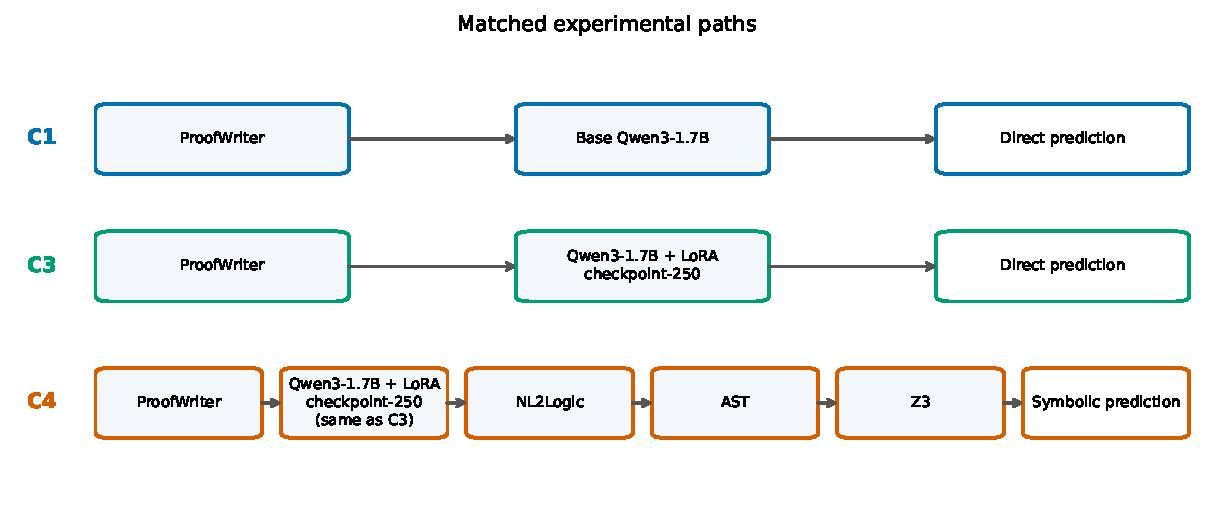
\includegraphics[width=0.96\textwidth]{figures/pipeline_overview.pdf}
\caption{Matched experimental paths. C3 and C4 use the same LoRA adapter \cite{lora} from checkpoint-250; only C4 adds the symbolic translation and solver path.}
\label{fig:pipeline}
\end{figure*}

\begin{table}[t]
\caption{Model and fine-tuning configuration.}
\label{tab:configuration}
\centering
\small
\begin{tabular}{ll}
\toprule
Item & Value \\
\midrule
Base model & Qwen3-1.7B \\
Quantization & NF4, FP16 compute \\
Training examples & 2,000 \\
Validation examples & 2,000 \\
LoRA rank / alpha / dropout & 16 / 32 / 0.05 \\
Learning rate / epochs & 2.0e-04 / 3 \\
Batch / accumulation & 1 / 16 \\
Optimizer / schedule & paged AdamW 8-bit / cosine \\
Selected adapter & checkpoint-250 \\
Bridge & descriptive NL2Logic $\rightarrow$ AST $\rightarrow$ Z3 \\
\bottomrule
\end{tabular}
\end{table}


\section{Experimental Setup}
\subsection{Data and canonical evidence}
The prepared ProofWriter source \cite{proofwriter} contains 585,552 training, 85,468 validation, and 174,476 test records. Controlled-language manifests select 2,000 training examples, 2,000 training-validation examples, and a 2,000-example held-out pool. The canonical evaluation is a label-and-QDep-stratified sample of 200 held-out examples using seed 42: 53 True, 53 False, and 94 Unknown. Table~\ref{tab:datasets} summarizes the splits.

The sole experimental source is the canonical ProofWriter run at \texttt{results/final200\_proofwriter}. Each condition contains 200 predictions with identical ordered identifiers, gold labels, and frozen subset hash. Provenance checks also require C3 and C4 to reference the same checkpoint-250 path; older and incomplete runs are excluded.

\begin{table}[t]
\caption{Dataset accounting. FOLIO is prepared but not evaluated.}
\label{tab:datasets}
\centering
\small
\begin{tabular}{lrrr}
\toprule
Dataset & Train & Validation & Held-out \\
\midrule
ProofWriter source & 585,552 & 85,468 & 174,476 \\
ProofWriter selected & 2,000 & 2,000 & 2,000 \\
ProofWriter canonical & -- & -- & 200 \\
FOLIO prepared & 896 & 105 & 203 \\
\bottomrule
\end{tabular}
\end{table}


\subsection{Metrics and statistical testing}
We report strict accuracy, macro precision/recall/F1, weighted F1, classwise scores, valid-output rate, and confusion matrices. Valid-only accuracy is reported only as a diagnostic and never replaces strict accuracy. For condition $c$ over $n=200$ examples,
\begin{equation}
\mathrm{Acc}_c=\frac{1}{n}\sum_{i=1}^{n}\mathbf{1}[\hat y_{c,i}=y_i].
\end{equation}
Confidence intervals use 10,000 paired bootstrap resamples with seed 42. The C3/C4 correctness difference is tested using the exact two-sided McNemar/binomial test on discordant pairs. The test concerns final correctness, not the internal cause of each error.

For intervention analysis we partition pairs into wrong$\rightarrow$correct (W$\rightarrow$C), correct$\rightarrow$correct, correct$\rightarrow$wrong (C$\rightarrow$W), and wrong$\rightarrow$wrong. The correction rate is W$\rightarrow$C divided by all C3 errors; the harm rate is C$\rightarrow$W divided by all C3 correct answers.

\subsection{Reproducibility}
Table~\ref{tab:configuration} lists the adaptation settings used for C3 and C4. Fine-tuning uses LoRA with rank 16, alpha 32, and dropout 0.05, a learning rate of $2.0\times10^{-4}$ for three epochs, per-device batch size 1 with gradient accumulation 16, and a paged 8-bit AdamW optimizer under a cosine schedule. The base model is loaded with NF4 quantization and FP16 compute in all conditions. Decoding is deterministic in C1 and C3, so repeated runs of the direct conditions reproduce the recorded predictions exactly.

Seed 42 governs both the stratified selection of the canonical 200-example subset and the 10,000 paired bootstrap resamples. The canonical subset is drawn from the 2,000-example held-out pool, which the split manifests keep separate from the 2,000 training and 2,000 training-validation examples.

%% TODO(authors): checkpoint-250 selection is NOT yet documented. Once the training
%% logs are available, state here (a) the criterion used to select step 250, (b) which
%% split the selection metric was computed on, and (c) that the canonical 200-example
%% held-out subset played no part in that selection. Do not assert (c) until the logs
%% confirm it. Required artifacts: trainer_state.json / training log with per-checkpoint
%% eval metrics, and the training config recording eval_dataset and save/eval strategy.
The criterion used to select checkpoint-250 is not documented in the current artifacts and is left for the camera-ready version. Per-example predictions, gold labels, and bridge traces for all three conditions are stored under \texttt{results/final200\_proofwriter}, and the reported tables, intervals, and figures are regenerated from those canonical predictions.

\section{Results}
\subsection{Fine-tuning effect: C1 to C3}
Table~\ref{tab:overall} and Fig.~\ref{fig:overall} show a large fine-tuning gain. Accuracy increases from 48.5\% (97/200) to 82.5\% (165/200), an absolute improvement of 34.0 percentage points. Macro-F1 increases from 0.251 to 0.826. The base model strongly defaults to Unknown: it achieves Unknown F1 of 0.646 but True F1 of 0.107 and False F1 of 0.000. Fine-tuning produces balanced classwise F1 scores of 0.854, 0.804, and 0.821 for True, False, and Unknown, respectively. Table~\ref{tab:perclass} reports per-class precision, recall, and F1 for all three conditions.

\begin{table*}[t]
\caption{Strict canonical ProofWriter results. Invalid outputs count as errors. Accuracy and validity are percentages.}
\label{tab:overall}
\centering
\small
\begin{tabular}{lrrrrr}
\toprule
Condition & Correct & Accuracy & Macro-F1 & Weighted F1 & Valid \\
\midrule
C1: base direct & 97/200 & 48.5 & 0.251 & 0.332 & 100.0 \\
C3: fine-tuned direct & 165/200 & \textbf{82.5} & \textbf{0.826} & 0.825 & 100.0 \\
C4: fine-tuned bridge & 99/200 & 49.5 & 0.459 & 0.491 & 89.5 \\
\bottomrule
\end{tabular}
\end{table*}


\begin{figure*}[t]
\centering
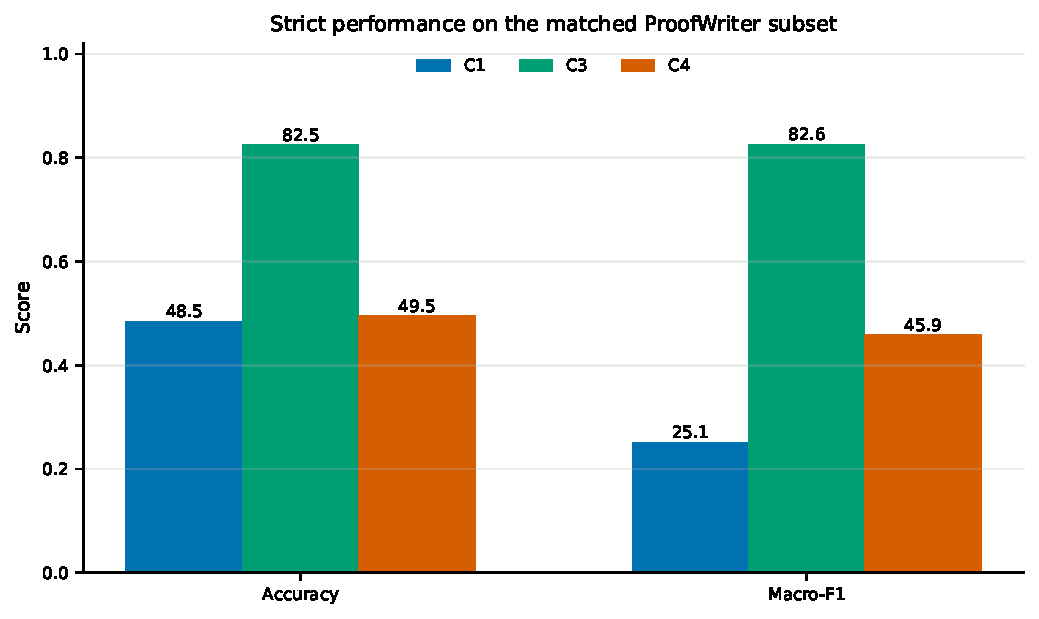
\includegraphics[width=0.78\textwidth]{figures/overall_comparison.pdf}
\caption{Strict accuracy and macro-F1. C1$\rightarrow$C3 isolates fine-tuning; C3$\rightarrow$C4 isolates the bridge.}
\label{fig:overall}
\end{figure*}

\begin{table}[t]
\caption{Per-class strict performance.}
\label{tab:perclass}
\centering
\scriptsize
\setlength{\tabcolsep}{3.2pt}
\begin{tabular}{llrrrr}
\toprule
Cond. & Class & Prec. & Rec. & F1 & Support \\
\midrule
C1 & True & 1.000 & 0.057 & 0.107 & 53 \\
C1 & False & 0.000 & 0.000 & 0.000 & 53 \\
C1 & Unknown & 0.477 & 1.000 & 0.646 & 94 \\
C3 & True & 0.880 & 0.830 & 0.854 & 53 \\
C3 & False & 0.837 & 0.774 & 0.804 & 53 \\
C3 & Unknown & 0.792 & 0.851 & 0.821 & 94 \\
C4 & True & 0.500 & 0.321 & 0.391 & 53 \\
C4 & False & 1.000 & 0.226 & 0.369 & 53 \\
C4 & Unknown & 0.526 & 0.745 & 0.617 & 94 \\
\bottomrule
\end{tabular}
\end{table}


\subsection{Bridge effect: C3 to C4}
Routing the same checkpoint through the bridge reduces strict accuracy from 82.5\% to 49.5\%, a 33.0-point decrease. Macro-F1 falls by 0.367, from 0.826 to 0.459. The paired bootstrap 95\% confidence interval for the accuracy difference is $[-0.410,-0.245]$, and exact McNemar testing on 90 discordant pairs gives $p=5.20\times10^{-13}$ (Table~\ref{tab:statistics}). The direct model makes 35 errors; C4 makes 101, corresponding to a 188.6\% increase in the error rate. C1 and C4 differ by only one accuracy point, but that contrast is descriptive because both adaptation and inference path differ.

C4 produces a valid label for 179 examples (89.5\%). Conditional accuracy on those valid outputs is 55.3\%, still far below C3. Thus, invalid outputs explain 21 errors but not the majority of the 66 additional errors.

\begin{table}[t]
\caption{Bootstrap intervals (10,000 paired resamples).}
\label{tab:statistics}
\centering
\scriptsize
\begin{tabular}{lrr}
\toprule
Quantity & Estimate & 95\% CI \\
\midrule
C1 accuracy & 0.485 & [0.415, 0.555] \\
C1 macro-F1 & 0.251 & [0.208, 0.299] \\
C3 accuracy & 0.825 & [0.770, 0.875] \\
C3 macro-F1 & 0.826 & [0.769, 0.876] \\
C4 accuracy & 0.495 & [0.430, 0.565] \\
C4 macro-F1 & 0.459 & [0.380, 0.534] \\
C4$-$C3 accuracy & -0.330 & [-0.410, -0.245] \\
\midrule
McNemar discordant & 90 & $p=5.20e-13$ \\
\bottomrule
\end{tabular}
\end{table}


\subsection{Confusion structure and reasoning depth}
Figure~\ref{fig:confusions} shows that C3 resolves True and False with few cross-class mistakes, while C4 shifts many cases toward Unknown: 29 of 53 True and 34 of 53 False instances become Unknown. C4 also maps 14 Unknown examples to True and yields 21 invalid predictions. This pattern is consistent with information being lost or distorted before symbolic inference.

\begin{figure*}[t]
\centering
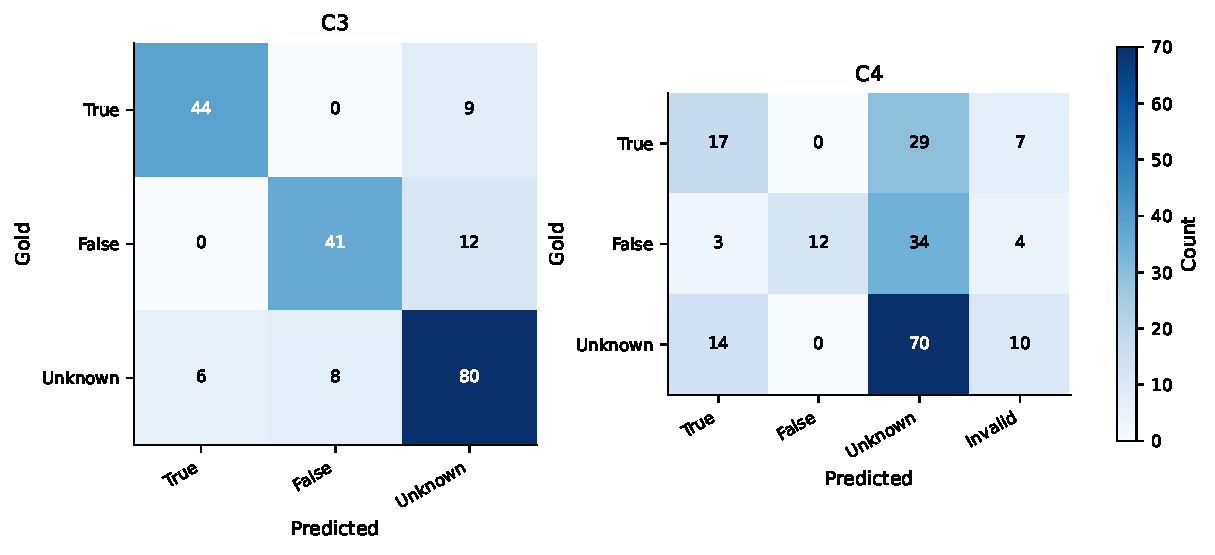
\includegraphics[width=0.90\textwidth]{figures/confusion_matrices.pdf}
\caption{Strict confusion matrices for C3 and C4. Invalid is a prediction outcome, not a fourth gold class.}
\label{fig:confusions}
\end{figure*}

QDep metadata support an observational depth analysis. C3 leads at every grouped depth: it moves from 96.2\% at depth 0 to 26.7\% at depth 3 and 75.0\% in the four-example 4+ group. C4 moves from 69.2\% at depth 0 to 6.7\% at depth 3 and 0\% at 4+. The imbalanced and very small tail groups preclude causal conclusions.

\section{Intervention and Error Analysis}
\subsection{Corrections versus harmful overturns}
The paired transition counts in Table~\ref{tab:interventions} reveal why aggregate performance collapses. C4 corrects 12 of C3's 35 errors, a 34.3\% correction rate. However, it overturns 78 of C3's 165 correct answers, a 47.3\% harm rate. Eighty-seven examples remain correct and 23 remain wrong, yielding 66 net lost corrections. A useful bridge policy would need to identify when translation and symbolic execution are trustworthy; no such policy exists in this implementation.

\begin{table}[t]
\caption{Paired C3$\rightarrow$C4 intervention outcomes.}
\label{tab:interventions}
\centering
\small
\begin{tabular}{lr}
\toprule
Outcome & Count \\
\midrule
Wrong $\rightarrow$ correct & 12 \\
Correct $\rightarrow$ correct & 87 \\
Correct $\rightarrow$ wrong & 78 \\
Wrong $\rightarrow$ wrong & 23 \\
\midrule
Correction rate & 34.3\% \\
Harm rate & 47.3\% \\
Net corrections & -66 \\
\bottomrule
\end{tabular}
\end{table}


\subsection{Levels of validity}
Bridge outcomes separate into distinct levels, and the canonical run lets us count where examples survive each one. Of 200 examples, 189 are syntactically well-formed; 180 of those are also schema and AST valid, and all 180 compile; 179 of the compiled representations are executable by Z3, with one rejected as an inconsistent premise set. Semantic correctness is not implied by any of these levels: across the run, exact and normalized logic matches against the reference interpretation are both zero, and the recorded semantic equivalence field is \texttt{different} for 158 examples. Final-answer correctness is lower still, at 99 of 200.

The gap between the 179 executable representations and the 99 correct final answers is the central observation of this section. Executability is a property of the form of a representation, whereas correctness of the final verdict additionally requires that the representation mean what the source theory meant. An executable symbolic representation can therefore be semantically wrong, and in this run most incorrect verdicts arise in exactly that case rather than from solver failure.

\subsection{Bridge outcome categories}
Table~\ref{tab:outcomes} groups the 200 examples by the stage of the pipeline at which the recorded fields place each outcome. These are pipeline outcome categories, not semantic error types: they record where an example stopped or what final verdict it received, and they do not identify which aspect of a translation was wrong. A classification of semantic error types would require per-example comparison of generated logical forms against reference interpretations, which the recorded fields do not support.

\begin{table}[t]
\caption{Bridge outcome categories for C4 ($n=200$), grouped by pipeline stage. These are outcome categories, not semantic error types.}
\label{tab:outcomes}
\centering
\small
\begin{tabular}{lrr}
\toprule
Category & Count & Rate (\%) \\
\midrule
Parser failure (malformed output) & 11 & 5.5 \\
Schema/AST invalid & 9 & 4.5 \\
Inconsistent premise set & 1 & 0.5 \\
Executable, incorrect final verdict & 80 & 40.0 \\
Executable, correct verdict & 99 & 49.5 \\
\bottomrule
\end{tabular}
\end{table}

\subsection{Bridge reliability and failure modes}
Table~\ref{tab:bridge} reports stage-level bridge outcomes. Twenty C4 examples fail before being run by a solver: 11 are malformed and nine are schema invalid. Of the remaining 180, 179 execute successfully in Z3 and one returns inconsistent premises. Yet, 80 of the 179 executable examples (44.7\% of executable cases; 40.0\% of all 200) return an incorrect symbolic conclusion.

Translation diagnostics yield direct evidence of mismatch. The recorded semantic equivalence field is \texttt{different} for 158 examples and unavailable for 42; exact and normalized logic matches are both zero. Parser recovery fields appear in 1,122 steps of trace data for 193 examples. These are step-level recovery events (not 1,122 failed examples), but the prevalence of permissive fallback behavior in the translation path is evident. We do not attribute every executable error to a particular parser step. Candidate mechanisms such as hypothesis mistranslation, rule mistranslation, predicate-argument inconsistency, and negation or variable-binding errors are not separately recorded in the available fields, and each can produce the same observable symptom of a solver-correct verdict over semantically altered logic. We therefore report the levels the traces do distinguish and treat the finer categories as candidate mechanisms rather than as measured frequencies.

\begin{table}[t]
\caption{C4 bridge reliability and outcomes ($n=200$).}
\label{tab:bridge}
\centering
\small
\begin{tabular}{lrr}
\toprule
Stage/outcome & Count & Rate (\%) \\
\midrule
Schema/parser/AST valid & 180 & 90.0 \\
Compilation success & 180 & 90.0 \\
Z3 executable & 179 & 89.5 \\
Correct symbolic verdict & 99 & 49.5 \\
Executable but incorrect & 80 & 40.0 \\
Malformed/schema invalid & 20 & 10.0 \\
Inconsistent premises & 1 & 0.5 \\
\bottomrule
\end{tabular}
\end{table}


\subsection{Latency}
Direct inference is inexpensive: mean end-to-end latency is 0.136 seconds for C1 and 0.228 seconds for C3. C4 averages 22.60 seconds (median 21.27, 95th percentile 38.71), about 99 times C3 latency. Across the 200 examples, C4 consumes roughly 75.3 minutes and records 11,726 recursive parser call requests and 3,960 model invocations. The current bridge therefore trades both accuracy and latency for symbolic executability.

\section{Discussion}
The C1/C3 comparison shows that it is the 2,000-example LoRA adaptation that is the dominant positive contributor in this experiment: it eliminates C1's strong Unknown bias in favor of balanced True/False/Unknown performance. The matched C3/C4 comparison then attributes the degradation to the added translation and symbolic inference pipeline rather than to a differing checkpoint.

The bridge is not uniformly detrimental---it fixes 12 errors---but its 78 harmful overturns suggest that the current translator is unable to reliably determine when its formalization has preserved the source theory. Future work should consider semantic consistency, predicate/variable binding, and calibrated abstention as novel matched conditions. This conclusion is specific to the implemented bridging mechanism and should not be construed as a general statement about the negative impact of neuro-symbolic components on reasoning.

\section{Limitations and Threats to Validity}
The canonical subset contains 200 examples from one controlled benchmark and one random seed. Although matched design supports paired inference, confidence intervals remain wide for small depth groups. ProofWriter's synthetic language limits generalization to naturally occurring text. The base model, adapter, prompts, and bridge are single implementations; results do not establish that fine-tuning always dominates neuro-symbolic reasoning or that NL2Logic generally fails.

The trace fields can establish well-formedness, execution, fallback activity, and recorded semantic mismatch, but they cannot uniquely assign causal responsibility for every incorrect verdict. Moreover, C4 has no retain/correct/abstain policy, so this study evaluates complete routing through the bridge rather than selective verification.

An additional natural-language benchmark is prepared for future work, but no matched prediction-level evaluation exists; no performance is reported. No matched self-check or symbolic-only baseline is available.

\section{Conclusion}
In a matched evaluation using 200 examples of ProofWriter, the accuracy of Qwen3-1.7B is increased from 48.5\% to 82.5\% by means of LoRA fine-tuning. When the same checkpoint is passed through the symbolic bridge that has been implemented, accuracy drops to 49.5\%. The bridge rectifies 12 direct errors but causes 78 answers which were originally correct to become incorrect; parser failures account for 20 of the invalid cases, while many of the executable verdicts are still wrong. Trace evidence suggests that translation fidelity, rather than symbolic reasoning in general, is a major bottleneck in this implementation.

\section*{Future Work}
Future work should be directed at enhancing the semantic fidelity during the NL2Logic translation phase before carrying out symbolic inference. Possible approaches might involve constrained decoding, explicit checks on predicates and variable bindings, stronger validation of the generated logical forms, and calibrated abstention when translation confidence is low. It could also be investigated to apply a selective verification policy so that symbolic reasoning is used only when the formalisation is sufficiently reliable, rather than always substituting the direct prediction from the model. The matched evaluation should also be extended to include FOLIO and other natural-language reasoning benchmarks to determine whether the failure modes observed with ProofWriter generalise beyond that system.
\bibliographystyle{IEEEtran}
\bibliography{references}

\end{document}
